\documentclass[twoside]{book}

% Packages required by doxygen
\usepackage{fixltx2e}
\usepackage{calc}
\usepackage{doxygen}
\usepackage[export]{adjustbox} % also loads graphicx
\usepackage{graphicx}
\usepackage[utf8]{inputenc}
\usepackage{makeidx}
\usepackage{multicol}
\usepackage{multirow}
\PassOptionsToPackage{warn}{textcomp}
\usepackage{textcomp}
\usepackage[nointegrals]{wasysym}
\usepackage[table]{xcolor}

% Font selection
\usepackage[T1]{fontenc}
\usepackage[scaled=.90]{helvet}
\usepackage{courier}
\usepackage{amssymb}
\usepackage{sectsty}
\renewcommand{\familydefault}{\sfdefault}
\allsectionsfont{%
  \fontseries{bc}\selectfont%
  \color{darkgray}%
}
\renewcommand{\DoxyLabelFont}{%
  \fontseries{bc}\selectfont%
  \color{darkgray}%
}
\newcommand{\+}{\discretionary{\mbox{\scriptsize$\hookleftarrow$}}{}{}}

% Page & text layout
\usepackage{geometry}
\geometry{%
  a4paper,%
  top=2.5cm,%
  bottom=2.5cm,%
  left=2.5cm,%
  right=2.5cm%
}
\tolerance=750
\hfuzz=15pt
\hbadness=750
\setlength{\emergencystretch}{15pt}
\setlength{\parindent}{0cm}
\setlength{\parskip}{3ex plus 2ex minus 2ex}
\makeatletter
\renewcommand{\paragraph}{%
  \@startsection{paragraph}{4}{0ex}{-1.0ex}{1.0ex}{%
    \normalfont\normalsize\bfseries\SS@parafont%
  }%
}
\renewcommand{\subparagraph}{%
  \@startsection{subparagraph}{5}{0ex}{-1.0ex}{1.0ex}{%
    \normalfont\normalsize\bfseries\SS@subparafont%
  }%
}
\makeatother

% Headers & footers
\usepackage{fancyhdr}
\pagestyle{fancyplain}
\fancyhead[LE]{\fancyplain{}{\bfseries\thepage}}
\fancyhead[CE]{\fancyplain{}{}}
\fancyhead[RE]{\fancyplain{}{\bfseries\leftmark}}
\fancyhead[LO]{\fancyplain{}{\bfseries\rightmark}}
\fancyhead[CO]{\fancyplain{}{}}
\fancyhead[RO]{\fancyplain{}{\bfseries\thepage}}
\fancyfoot[LE]{\fancyplain{}{}}
\fancyfoot[CE]{\fancyplain{}{}}
\fancyfoot[RE]{\fancyplain{}{\bfseries\scriptsize Generated by Doxygen }}
\fancyfoot[LO]{\fancyplain{}{\bfseries\scriptsize Generated by Doxygen }}
\fancyfoot[CO]{\fancyplain{}{}}
\fancyfoot[RO]{\fancyplain{}{}}
\renewcommand{\footrulewidth}{0.4pt}
\renewcommand{\chaptermark}[1]{%
  \markboth{#1}{}%
}
\renewcommand{\sectionmark}[1]{%
  \markright{\thesection\ #1}%
}

% Indices & bibliography
\usepackage{natbib}
\usepackage[titles]{tocloft}
\setcounter{tocdepth}{3}
\setcounter{secnumdepth}{5}
\makeindex

% Hyperlinks (required, but should be loaded last)
\usepackage{ifpdf}
\ifpdf
  \usepackage[pdftex,pagebackref=true]{hyperref}
\else
  \usepackage[ps2pdf,pagebackref=true]{hyperref}
\fi
\hypersetup{%
  colorlinks=true,%
  linkcolor=blue,%
  citecolor=blue,%
  unicode%
}

% Custom commands
\newcommand{\clearemptydoublepage}{%
  \newpage{\pagestyle{empty}\cleardoublepage}%
}

\usepackage{caption}
\captionsetup{labelsep=space,justification=centering,font={bf},singlelinecheck=off,skip=4pt,position=top}

%===== C O N T E N T S =====

\begin{document}

% Titlepage & ToC
\hypersetup{pageanchor=false,
             bookmarksnumbered=true,
             pdfencoding=unicode
            }
\pagenumbering{alph}
\begin{titlepage}
\vspace*{7cm}
\begin{center}%
{\Large Data Structures -\/ Linked\+List -\/ Doc\+Test \\[1ex]\large 0.\+001 }\\
\vspace*{1cm}
{\large Generated by Doxygen 1.8.13}\\
\end{center}
\end{titlepage}
\clearemptydoublepage
\pagenumbering{roman}
\tableofcontents
\clearemptydoublepage
\pagenumbering{arabic}
\hypersetup{pageanchor=true}

%--- Begin generated contents ---
\chapter{Class Index}
\section{Class List}
Here are the classes, structs, unions and interfaces with brief descriptions\+:\begin{DoxyCompactList}
\item\contentsline{section}{\hyperlink{class_linked_list}{Linked\+List} }{\pageref{class_linked_list}}{}
\item\contentsline{section}{\hyperlink{class_node}{Node} }{\pageref{class_node}}{}
\end{DoxyCompactList}

\chapter{File Index}
\section{File List}
Here is a list of all files with brief descriptions\+:\begin{DoxyCompactList}
\item\contentsline{section}{D\+:/\+Git/\+Data\+Structures/\+Linked\+List/\hyperlink{_list_8cpp}{List.\+cpp} }{\pageref{_list_8cpp}}{}
\item\contentsline{section}{D\+:/\+Git/\+Data\+Structures/\+Linked\+List/\hyperlink{_list_8hpp}{List.\+hpp} }{\pageref{_list_8hpp}}{}
\item\contentsline{section}{D\+:/\+Git/\+Data\+Structures/\+Linked\+List/\hyperlink{main_8cpp}{main.\+cpp} }{\pageref{main_8cpp}}{}
\item\contentsline{section}{D\+:/\+Git/\+Data\+Structures/\+Linked\+List/\hyperlink{_node_8cpp}{Node.\+cpp} }{\pageref{_node_8cpp}}{}
\item\contentsline{section}{D\+:/\+Git/\+Data\+Structures/\+Linked\+List/\hyperlink{_node_8hpp}{Node.\+hpp} }{\pageref{_node_8hpp}}{}
\end{DoxyCompactList}

\chapter{Class Documentation}
\hypertarget{class_linked_list}{}\section{Linked\+List Class Reference}
\label{class_linked_list}\index{Linked\+List@{Linked\+List}}


{\ttfamily \#include $<$List.\+hpp$>$}

\subsection*{Public Member Functions}
\begin{DoxyCompactItemize}
\item 
\hyperlink{class_linked_list_afe7f78983e173f8018927cf2ad11a5aa}{Linked\+List} ()
\item 
\hyperlink{class_linked_list_ae4a0a3646caae0f7eedb6bd6d6744dbb}{Linked\+List} (\hyperlink{class_node}{Node} $\ast$head)
\item 
\hyperlink{class_linked_list_a5dd2a88ad50e83aee19dea51c8d87d90}{Linked\+List} (const \hyperlink{class_linked_list}{Linked\+List} \&head)
\item 
\hyperlink{class_linked_list_a35811ed58ff0d8d9cc9b309b8d8f5111}{$\sim$\+Linked\+List} ()
\item 
void \hyperlink{class_linked_list_a583e4bb42bb128feddb57767863fd28e}{insert\+Beg} (int data)
\item 
void \hyperlink{class_linked_list_af508f8b52bbcf1485a1552ac8fc84b81}{insert\+After} (int data, \hyperlink{class_node}{Node} $\ast$key\+\_\+node)
\item 
void \hyperlink{class_linked_list_a895ad950cc619c9cf72273e5e59a100f}{insert\+Before} (int data, \hyperlink{class_node}{Node} $\ast$key\+\_\+node)
\item 
void \hyperlink{class_linked_list_a8b87744316967b16f272be10cd6718ed}{insert\+End} (int data)
\item 
void \hyperlink{class_linked_list_a2e67fa8d36b83febafbd5f3801ec43db}{append} (\hyperlink{class_node}{Node} $\ast$)
\item 
void \hyperlink{class_linked_list_af8ccdfe634eed9feae0c641766e2e867}{delete\+Beg} ()
\item 
void \hyperlink{class_linked_list_a9a53a4d26d1c757f3d526db3fa43c2f8}{delete\+Node} (\hyperlink{class_node}{Node} $\ast$key\+\_\+node)
\item 
void \hyperlink{class_linked_list_ab624ff78c70aaa517a3a98a4e7fec288}{delete\+End} ()
\item 
int \hyperlink{class_linked_list_a8b00d7145aa7ee83ba2e49623285e371}{delete\+All} (int key)
\item 
void \hyperlink{class_linked_list_a2d03b30bf762af404a7a687aceff7123}{print\+ListR} (\hyperlink{class_node}{Node} $\ast$tmp)
\item 
void \hyperlink{class_linked_list_ac96230938fd74a4efeb4efe8c995ee53}{print\+List} ()
\item 
size\+\_\+t \hyperlink{class_linked_list_af4b27646ebfb44d2fd0625b8ad1fb136}{get\+SizeR} (\hyperlink{class_node}{Node} $\ast$tmp)
\item 
size\+\_\+t \hyperlink{class_linked_list_ac8d24166208694f4fe3cc982307b03fb}{get\+Size} ()
\item 
\hyperlink{class_node}{Node} $\ast$ \hyperlink{class_linked_list_a1cba1fc059374f4d263bf5bece9fa136}{get\+Head} ()
\item 
\hyperlink{class_node}{Node} $\ast$ \hyperlink{class_linked_list_a744fc291de7eff0b934e7b594449fa10}{get\+First} ()
\item 
\hyperlink{class_node}{Node} $\ast$ \hyperlink{class_linked_list_ad07d8659b87f77e9fb98a80eb71ed77a}{get\+Last} ()
\item 
bool \hyperlink{class_linked_list_a03ff22f881325da2d37f640ab2380bf2}{is\+Empty} ()
\item 
bool \hyperlink{class_linked_list_a1a5c8f3b415fa55f7e876cf4a01f3380}{is\+Not\+Empty} ()
\item 
int \hyperlink{class_linked_list_a2866982bfe5f87a2a265d1e2ec3e43ed}{get\+Element} (int pos)
\item 
bool \hyperlink{class_linked_list_ac2fac6f86f1891576b57c2866ff77803}{contains} (int key)
\item 
bool \hyperlink{class_linked_list_a67c86ff482738c1ab36bb8c764a7f3f7}{containsR} (\hyperlink{class_node}{Node} $\ast$tmp, int key)
\item 
void \hyperlink{class_linked_list_ac517f07c7f197202fa085246fb3f07e8}{insert\+Sorted} (\hyperlink{class_node}{Node} $\ast$$\ast$sorted, int key)
\item 
void \hyperlink{class_linked_list_a04e277f98f8e6e5426f19ad780915e00}{insertion\+Sort} ()
\end{DoxyCompactItemize}


\subsection{Constructor \& Destructor Documentation}
\mbox{\Hypertarget{class_linked_list_afe7f78983e173f8018927cf2ad11a5aa}\label{class_linked_list_afe7f78983e173f8018927cf2ad11a5aa}} 
\index{Linked\+List@{Linked\+List}!Linked\+List@{Linked\+List}}
\index{Linked\+List@{Linked\+List}!Linked\+List@{Linked\+List}}
\subsubsection{\texorpdfstring{Linked\+List()}{LinkedList()}\hspace{0.1cm}{\footnotesize\ttfamily [1/3]}}
{\footnotesize\ttfamily Linked\+List\+::\+Linked\+List (\begin{DoxyParamCaption}{ }\end{DoxyParamCaption})}

\mbox{\Hypertarget{class_linked_list_ae4a0a3646caae0f7eedb6bd6d6744dbb}\label{class_linked_list_ae4a0a3646caae0f7eedb6bd6d6744dbb}} 
\index{Linked\+List@{Linked\+List}!Linked\+List@{Linked\+List}}
\index{Linked\+List@{Linked\+List}!Linked\+List@{Linked\+List}}
\subsubsection{\texorpdfstring{Linked\+List()}{LinkedList()}\hspace{0.1cm}{\footnotesize\ttfamily [2/3]}}
{\footnotesize\ttfamily Linked\+List\+::\+Linked\+List (\begin{DoxyParamCaption}\item[{\hyperlink{class_node}{Node} $\ast$}]{head }\end{DoxyParamCaption})}

\mbox{\Hypertarget{class_linked_list_a5dd2a88ad50e83aee19dea51c8d87d90}\label{class_linked_list_a5dd2a88ad50e83aee19dea51c8d87d90}} 
\index{Linked\+List@{Linked\+List}!Linked\+List@{Linked\+List}}
\index{Linked\+List@{Linked\+List}!Linked\+List@{Linked\+List}}
\subsubsection{\texorpdfstring{Linked\+List()}{LinkedList()}\hspace{0.1cm}{\footnotesize\ttfamily [3/3]}}
{\footnotesize\ttfamily Linked\+List\+::\+Linked\+List (\begin{DoxyParamCaption}\item[{const \hyperlink{class_linked_list}{Linked\+List} \&}]{head }\end{DoxyParamCaption})}

Here is the call graph for this function\+:
% FIG 0
\mbox{\Hypertarget{class_linked_list_a35811ed58ff0d8d9cc9b309b8d8f5111}\label{class_linked_list_a35811ed58ff0d8d9cc9b309b8d8f5111}} 
\index{Linked\+List@{Linked\+List}!````~Linked\+List@{$\sim$\+Linked\+List}}
\index{````~Linked\+List@{$\sim$\+Linked\+List}!Linked\+List@{Linked\+List}}
\subsubsection{\texorpdfstring{$\sim$\+Linked\+List()}{~LinkedList()}}
{\footnotesize\ttfamily Linked\+List\+::$\sim$\+Linked\+List (\begin{DoxyParamCaption}{ }\end{DoxyParamCaption})}



\subsection{Member Function Documentation}
\mbox{\Hypertarget{class_linked_list_a2e67fa8d36b83febafbd5f3801ec43db}\label{class_linked_list_a2e67fa8d36b83febafbd5f3801ec43db}} 
\index{Linked\+List@{Linked\+List}!append@{append}}
\index{append@{append}!Linked\+List@{Linked\+List}}
\subsubsection{\texorpdfstring{append()}{append()}}
{\footnotesize\ttfamily void Linked\+List\+::append (\begin{DoxyParamCaption}\item[{\hyperlink{class_node}{Node} $\ast$}]{node }\end{DoxyParamCaption})}

Here is the call graph for this function\+:
% FIG 1
Here is the caller graph for this function\+:
% FIG 2
\mbox{\Hypertarget{class_linked_list_ac2fac6f86f1891576b57c2866ff77803}\label{class_linked_list_ac2fac6f86f1891576b57c2866ff77803}} 
\index{Linked\+List@{Linked\+List}!contains@{contains}}
\index{contains@{contains}!Linked\+List@{Linked\+List}}
\subsubsection{\texorpdfstring{contains()}{contains()}}
{\footnotesize\ttfamily bool Linked\+List\+::contains (\begin{DoxyParamCaption}\item[{int}]{key }\end{DoxyParamCaption})}

Here is the call graph for this function\+:
% FIG 3
Here is the caller graph for this function\+:
% FIG 4
\mbox{\Hypertarget{class_linked_list_a67c86ff482738c1ab36bb8c764a7f3f7}\label{class_linked_list_a67c86ff482738c1ab36bb8c764a7f3f7}} 
\index{Linked\+List@{Linked\+List}!containsR@{containsR}}
\index{containsR@{containsR}!Linked\+List@{Linked\+List}}
\subsubsection{\texorpdfstring{contains\+R()}{containsR()}}
{\footnotesize\ttfamily bool Linked\+List\+::containsR (\begin{DoxyParamCaption}\item[{\hyperlink{class_node}{Node} $\ast$}]{tmp,  }\item[{int}]{key }\end{DoxyParamCaption})}

Here is the call graph for this function\+:
% FIG 5
Here is the caller graph for this function\+:
% FIG 6
\mbox{\Hypertarget{class_linked_list_a8b00d7145aa7ee83ba2e49623285e371}\label{class_linked_list_a8b00d7145aa7ee83ba2e49623285e371}} 
\index{Linked\+List@{Linked\+List}!delete\+All@{delete\+All}}
\index{delete\+All@{delete\+All}!Linked\+List@{Linked\+List}}
\subsubsection{\texorpdfstring{delete\+All()}{deleteAll()}}
{\footnotesize\ttfamily int Linked\+List\+::delete\+All (\begin{DoxyParamCaption}\item[{int}]{key }\end{DoxyParamCaption})}

Here is the call graph for this function\+:
% FIG 7
Here is the caller graph for this function\+:
% FIG 8
\mbox{\Hypertarget{class_linked_list_af8ccdfe634eed9feae0c641766e2e867}\label{class_linked_list_af8ccdfe634eed9feae0c641766e2e867}} 
\index{Linked\+List@{Linked\+List}!delete\+Beg@{delete\+Beg}}
\index{delete\+Beg@{delete\+Beg}!Linked\+List@{Linked\+List}}
\subsubsection{\texorpdfstring{delete\+Beg()}{deleteBeg()}}
{\footnotesize\ttfamily void Linked\+List\+::delete\+Beg (\begin{DoxyParamCaption}{ }\end{DoxyParamCaption})}

Here is the call graph for this function\+:
% FIG 9
Here is the caller graph for this function\+:
% FIG 10
\mbox{\Hypertarget{class_linked_list_ab624ff78c70aaa517a3a98a4e7fec288}\label{class_linked_list_ab624ff78c70aaa517a3a98a4e7fec288}} 
\index{Linked\+List@{Linked\+List}!delete\+End@{delete\+End}}
\index{delete\+End@{delete\+End}!Linked\+List@{Linked\+List}}
\subsubsection{\texorpdfstring{delete\+End()}{deleteEnd()}}
{\footnotesize\ttfamily void Linked\+List\+::delete\+End (\begin{DoxyParamCaption}{ }\end{DoxyParamCaption})}

Here is the call graph for this function\+:
% FIG 11
Here is the caller graph for this function\+:
% FIG 12
\mbox{\Hypertarget{class_linked_list_a9a53a4d26d1c757f3d526db3fa43c2f8}\label{class_linked_list_a9a53a4d26d1c757f3d526db3fa43c2f8}} 
\index{Linked\+List@{Linked\+List}!delete\+Node@{delete\+Node}}
\index{delete\+Node@{delete\+Node}!Linked\+List@{Linked\+List}}
\subsubsection{\texorpdfstring{delete\+Node()}{deleteNode()}}
{\footnotesize\ttfamily void Linked\+List\+::delete\+Node (\begin{DoxyParamCaption}\item[{\hyperlink{class_node}{Node} $\ast$}]{key\+\_\+node }\end{DoxyParamCaption})}

Here is the call graph for this function\+:
% FIG 13
Here is the caller graph for this function\+:
% FIG 14
\mbox{\Hypertarget{class_linked_list_a2866982bfe5f87a2a265d1e2ec3e43ed}\label{class_linked_list_a2866982bfe5f87a2a265d1e2ec3e43ed}} 
\index{Linked\+List@{Linked\+List}!get\+Element@{get\+Element}}
\index{get\+Element@{get\+Element}!Linked\+List@{Linked\+List}}
\subsubsection{\texorpdfstring{get\+Element()}{getElement()}}
{\footnotesize\ttfamily int Linked\+List\+::get\+Element (\begin{DoxyParamCaption}\item[{int}]{pos }\end{DoxyParamCaption})}

Here is the call graph for this function\+:
% FIG 15
Here is the caller graph for this function\+:
% FIG 16
\mbox{\Hypertarget{class_linked_list_a744fc291de7eff0b934e7b594449fa10}\label{class_linked_list_a744fc291de7eff0b934e7b594449fa10}} 
\index{Linked\+List@{Linked\+List}!get\+First@{get\+First}}
\index{get\+First@{get\+First}!Linked\+List@{Linked\+List}}
\subsubsection{\texorpdfstring{get\+First()}{getFirst()}}
{\footnotesize\ttfamily \hyperlink{class_node}{Node} $\ast$ Linked\+List\+::get\+First (\begin{DoxyParamCaption}{ }\end{DoxyParamCaption})\hspace{0.3cm}{\ttfamily [inline]}}

Here is the caller graph for this function\+:
% FIG 17
\mbox{\Hypertarget{class_linked_list_a1cba1fc059374f4d263bf5bece9fa136}\label{class_linked_list_a1cba1fc059374f4d263bf5bece9fa136}} 
\index{Linked\+List@{Linked\+List}!get\+Head@{get\+Head}}
\index{get\+Head@{get\+Head}!Linked\+List@{Linked\+List}}
\subsubsection{\texorpdfstring{get\+Head()}{getHead()}}
{\footnotesize\ttfamily \hyperlink{class_node}{Node} $\ast$ Linked\+List\+::get\+Head (\begin{DoxyParamCaption}{ }\end{DoxyParamCaption})}

Here is the caller graph for this function\+:
% FIG 18
\mbox{\Hypertarget{class_linked_list_ad07d8659b87f77e9fb98a80eb71ed77a}\label{class_linked_list_ad07d8659b87f77e9fb98a80eb71ed77a}} 
\index{Linked\+List@{Linked\+List}!get\+Last@{get\+Last}}
\index{get\+Last@{get\+Last}!Linked\+List@{Linked\+List}}
\subsubsection{\texorpdfstring{get\+Last()}{getLast()}}
{\footnotesize\ttfamily \hyperlink{class_node}{Node} $\ast$ Linked\+List\+::get\+Last (\begin{DoxyParamCaption}{ }\end{DoxyParamCaption})}

Here is the call graph for this function\+:
% FIG 19
Here is the caller graph for this function\+:
% FIG 20
\mbox{\Hypertarget{class_linked_list_ac8d24166208694f4fe3cc982307b03fb}\label{class_linked_list_ac8d24166208694f4fe3cc982307b03fb}} 
\index{Linked\+List@{Linked\+List}!get\+Size@{get\+Size}}
\index{get\+Size@{get\+Size}!Linked\+List@{Linked\+List}}
\subsubsection{\texorpdfstring{get\+Size()}{getSize()}}
{\footnotesize\ttfamily size\+\_\+t Linked\+List\+::get\+Size (\begin{DoxyParamCaption}{ }\end{DoxyParamCaption})}

Here is the call graph for this function\+:
% FIG 21
Here is the caller graph for this function\+:
% FIG 22
\mbox{\Hypertarget{class_linked_list_af4b27646ebfb44d2fd0625b8ad1fb136}\label{class_linked_list_af4b27646ebfb44d2fd0625b8ad1fb136}} 
\index{Linked\+List@{Linked\+List}!get\+SizeR@{get\+SizeR}}
\index{get\+SizeR@{get\+SizeR}!Linked\+List@{Linked\+List}}
\subsubsection{\texorpdfstring{get\+Size\+R()}{getSizeR()}}
{\footnotesize\ttfamily size\+\_\+t Linked\+List\+::get\+SizeR (\begin{DoxyParamCaption}\item[{\hyperlink{class_node}{Node} $\ast$}]{tmp }\end{DoxyParamCaption})}

Here is the call graph for this function\+:
% FIG 23
Here is the caller graph for this function\+:
% FIG 24
\mbox{\Hypertarget{class_linked_list_af508f8b52bbcf1485a1552ac8fc84b81}\label{class_linked_list_af508f8b52bbcf1485a1552ac8fc84b81}} 
\index{Linked\+List@{Linked\+List}!insert\+After@{insert\+After}}
\index{insert\+After@{insert\+After}!Linked\+List@{Linked\+List}}
\subsubsection{\texorpdfstring{insert\+After()}{insertAfter()}}
{\footnotesize\ttfamily void Linked\+List\+::insert\+After (\begin{DoxyParamCaption}\item[{int}]{data,  }\item[{\hyperlink{class_node}{Node} $\ast$}]{key\+\_\+node }\end{DoxyParamCaption})}

Here is the call graph for this function\+:
% FIG 25
Here is the caller graph for this function\+:
% FIG 26
\mbox{\Hypertarget{class_linked_list_a895ad950cc619c9cf72273e5e59a100f}\label{class_linked_list_a895ad950cc619c9cf72273e5e59a100f}} 
\index{Linked\+List@{Linked\+List}!insert\+Before@{insert\+Before}}
\index{insert\+Before@{insert\+Before}!Linked\+List@{Linked\+List}}
\subsubsection{\texorpdfstring{insert\+Before()}{insertBefore()}}
{\footnotesize\ttfamily void Linked\+List\+::insert\+Before (\begin{DoxyParamCaption}\item[{int}]{data,  }\item[{\hyperlink{class_node}{Node} $\ast$}]{key\+\_\+node }\end{DoxyParamCaption})}

Here is the call graph for this function\+:
% FIG 27
Here is the caller graph for this function\+:
% FIG 28
\mbox{\Hypertarget{class_linked_list_a583e4bb42bb128feddb57767863fd28e}\label{class_linked_list_a583e4bb42bb128feddb57767863fd28e}} 
\index{Linked\+List@{Linked\+List}!insert\+Beg@{insert\+Beg}}
\index{insert\+Beg@{insert\+Beg}!Linked\+List@{Linked\+List}}
\subsubsection{\texorpdfstring{insert\+Beg()}{insertBeg()}}
{\footnotesize\ttfamily void Linked\+List\+::insert\+Beg (\begin{DoxyParamCaption}\item[{int}]{data }\end{DoxyParamCaption})}

Here is the caller graph for this function\+:
% FIG 29
\mbox{\Hypertarget{class_linked_list_a8b87744316967b16f272be10cd6718ed}\label{class_linked_list_a8b87744316967b16f272be10cd6718ed}} 
\index{Linked\+List@{Linked\+List}!insert\+End@{insert\+End}}
\index{insert\+End@{insert\+End}!Linked\+List@{Linked\+List}}
\subsubsection{\texorpdfstring{insert\+End()}{insertEnd()}}
{\footnotesize\ttfamily void Linked\+List\+::insert\+End (\begin{DoxyParamCaption}\item[{int}]{data }\end{DoxyParamCaption})}

Here is the call graph for this function\+:
% FIG 30
Here is the caller graph for this function\+:
% FIG 31
\mbox{\Hypertarget{class_linked_list_a04e277f98f8e6e5426f19ad780915e00}\label{class_linked_list_a04e277f98f8e6e5426f19ad780915e00}} 
\index{Linked\+List@{Linked\+List}!insertion\+Sort@{insertion\+Sort}}
\index{insertion\+Sort@{insertion\+Sort}!Linked\+List@{Linked\+List}}
\subsubsection{\texorpdfstring{insertion\+Sort()}{insertionSort()}}
{\footnotesize\ttfamily void Linked\+List\+::insertion\+Sort (\begin{DoxyParamCaption}{ }\end{DoxyParamCaption})}

Here is the call graph for this function\+:
% FIG 32
Here is the caller graph for this function\+:
% FIG 33
\mbox{\Hypertarget{class_linked_list_ac517f07c7f197202fa085246fb3f07e8}\label{class_linked_list_ac517f07c7f197202fa085246fb3f07e8}} 
\index{Linked\+List@{Linked\+List}!insert\+Sorted@{insert\+Sorted}}
\index{insert\+Sorted@{insert\+Sorted}!Linked\+List@{Linked\+List}}
\subsubsection{\texorpdfstring{insert\+Sorted()}{insertSorted()}}
{\footnotesize\ttfamily void Linked\+List\+::insert\+Sorted (\begin{DoxyParamCaption}\item[{\hyperlink{class_node}{Node} $\ast$$\ast$}]{sorted,  }\item[{int}]{key }\end{DoxyParamCaption})}

Here is the call graph for this function\+:
% FIG 34
Here is the caller graph for this function\+:
% FIG 35
\mbox{\Hypertarget{class_linked_list_a03ff22f881325da2d37f640ab2380bf2}\label{class_linked_list_a03ff22f881325da2d37f640ab2380bf2}} 
\index{Linked\+List@{Linked\+List}!is\+Empty@{is\+Empty}}
\index{is\+Empty@{is\+Empty}!Linked\+List@{Linked\+List}}
\subsubsection{\texorpdfstring{is\+Empty()}{isEmpty()}}
{\footnotesize\ttfamily bool Linked\+List\+::is\+Empty (\begin{DoxyParamCaption}{ }\end{DoxyParamCaption})}

\mbox{\Hypertarget{class_linked_list_a1a5c8f3b415fa55f7e876cf4a01f3380}\label{class_linked_list_a1a5c8f3b415fa55f7e876cf4a01f3380}} 
\index{Linked\+List@{Linked\+List}!is\+Not\+Empty@{is\+Not\+Empty}}
\index{is\+Not\+Empty@{is\+Not\+Empty}!Linked\+List@{Linked\+List}}
\subsubsection{\texorpdfstring{is\+Not\+Empty()}{isNotEmpty()}}
{\footnotesize\ttfamily bool Linked\+List\+::is\+Not\+Empty (\begin{DoxyParamCaption}{ }\end{DoxyParamCaption})}

Here is the caller graph for this function\+:
% FIG 36
\mbox{\Hypertarget{class_linked_list_ac96230938fd74a4efeb4efe8c995ee53}\label{class_linked_list_ac96230938fd74a4efeb4efe8c995ee53}} 
\index{Linked\+List@{Linked\+List}!print\+List@{print\+List}}
\index{print\+List@{print\+List}!Linked\+List@{Linked\+List}}
\subsubsection{\texorpdfstring{print\+List()}{printList()}}
{\footnotesize\ttfamily void Linked\+List\+::print\+List (\begin{DoxyParamCaption}{ }\end{DoxyParamCaption})}

Here is the call graph for this function\+:
% FIG 37
Here is the caller graph for this function\+:
% FIG 38
\mbox{\Hypertarget{class_linked_list_a2d03b30bf762af404a7a687aceff7123}\label{class_linked_list_a2d03b30bf762af404a7a687aceff7123}} 
\index{Linked\+List@{Linked\+List}!print\+ListR@{print\+ListR}}
\index{print\+ListR@{print\+ListR}!Linked\+List@{Linked\+List}}
\subsubsection{\texorpdfstring{print\+List\+R()}{printListR()}}
{\footnotesize\ttfamily void Linked\+List\+::print\+ListR (\begin{DoxyParamCaption}\item[{\hyperlink{class_node}{Node} $\ast$}]{tmp }\end{DoxyParamCaption})}

Here is the call graph for this function\+:
% FIG 39
Here is the caller graph for this function\+:
% FIG 40


The documentation for this class was generated from the following files\+:\begin{DoxyCompactItemize}
\item 
D\+:/\+Git/\+Data\+Structures/\+Linked\+List/\hyperlink{_list_8hpp}{List.\+hpp}\item 
D\+:/\+Git/\+Data\+Structures/\+Linked\+List/\hyperlink{_list_8cpp}{List.\+cpp}\end{DoxyCompactItemize}

\hypertarget{class_node}{}\section{Node Class Reference}
\label{class_node}\index{Node@{Node}}


{\ttfamily \#include $<$Node.\+hpp$>$}

\subsection*{Public Member Functions}
\begin{DoxyCompactItemize}
\item 
\hyperlink{class_node_ad7a34779cad45d997bfd6d3d8043c75f}{Node} ()
\item 
\hyperlink{class_node_aff71d952af8363f046a67a8b12194e46}{Node} (int)
\item 
\hyperlink{class_node_aff31c12e14a6f00952a46ff967db0c96}{Node} (int, \hyperlink{class_node}{Node} $\ast$)
\item 
\hyperlink{class_node_a4053c6deca192c41824fad14c4f4eb76}{Node} (const \hyperlink{class_node}{Node} \&)
\item 
\hyperlink{class_node_aa0840c3cb5c7159be6d992adecd2097c}{$\sim$\+Node} ()
\item 
void \hyperlink{class_node_a0a2c821ab31b604e4fdd7cf39be5cc68}{set\+Data} (int)
\item 
void \hyperlink{class_node_a89b12aca90acdf6a8a547cbdab9b80a5}{set\+Next} (\hyperlink{class_node}{Node} $\ast$)
\item 
int \hyperlink{class_node_aca98907146d5d0687f48bf8be9df9b7d}{get\+Data} ()
\item 
\hyperlink{class_node}{Node} $\ast$ \hyperlink{class_node_ae36639ff267d63e058ce309fde5a9913}{get\+Next} ()
\end{DoxyCompactItemize}


\subsection{Constructor \& Destructor Documentation}
\mbox{\Hypertarget{class_node_ad7a34779cad45d997bfd6d3d8043c75f}\label{class_node_ad7a34779cad45d997bfd6d3d8043c75f}} 
\index{Node@{Node}!Node@{Node}}
\index{Node@{Node}!Node@{Node}}
\subsubsection{\texorpdfstring{Node()}{Node()}\hspace{0.1cm}{\footnotesize\ttfamily [1/4]}}
{\footnotesize\ttfamily Node\+::\+Node (\begin{DoxyParamCaption}{ }\end{DoxyParamCaption})}

\mbox{\Hypertarget{class_node_aff71d952af8363f046a67a8b12194e46}\label{class_node_aff71d952af8363f046a67a8b12194e46}} 
\index{Node@{Node}!Node@{Node}}
\index{Node@{Node}!Node@{Node}}
\subsubsection{\texorpdfstring{Node()}{Node()}\hspace{0.1cm}{\footnotesize\ttfamily [2/4]}}
{\footnotesize\ttfamily Node\+::\+Node (\begin{DoxyParamCaption}\item[{int}]{data }\end{DoxyParamCaption})}

\mbox{\Hypertarget{class_node_aff31c12e14a6f00952a46ff967db0c96}\label{class_node_aff31c12e14a6f00952a46ff967db0c96}} 
\index{Node@{Node}!Node@{Node}}
\index{Node@{Node}!Node@{Node}}
\subsubsection{\texorpdfstring{Node()}{Node()}\hspace{0.1cm}{\footnotesize\ttfamily [3/4]}}
{\footnotesize\ttfamily Node\+::\+Node (\begin{DoxyParamCaption}\item[{int}]{data,  }\item[{\hyperlink{class_node}{Node} $\ast$}]{next }\end{DoxyParamCaption})}

\mbox{\Hypertarget{class_node_a4053c6deca192c41824fad14c4f4eb76}\label{class_node_a4053c6deca192c41824fad14c4f4eb76}} 
\index{Node@{Node}!Node@{Node}}
\index{Node@{Node}!Node@{Node}}
\subsubsection{\texorpdfstring{Node()}{Node()}\hspace{0.1cm}{\footnotesize\ttfamily [4/4]}}
{\footnotesize\ttfamily Node\+::\+Node (\begin{DoxyParamCaption}\item[{const \hyperlink{class_node}{Node} \&}]{node }\end{DoxyParamCaption})}

\mbox{\Hypertarget{class_node_aa0840c3cb5c7159be6d992adecd2097c}\label{class_node_aa0840c3cb5c7159be6d992adecd2097c}} 
\index{Node@{Node}!````~Node@{$\sim$\+Node}}
\index{````~Node@{$\sim$\+Node}!Node@{Node}}
\subsubsection{\texorpdfstring{$\sim$\+Node()}{~Node()}}
{\footnotesize\ttfamily Node\+::$\sim$\+Node (\begin{DoxyParamCaption}{ }\end{DoxyParamCaption})}



\subsection{Member Function Documentation}
\mbox{\Hypertarget{class_node_aca98907146d5d0687f48bf8be9df9b7d}\label{class_node_aca98907146d5d0687f48bf8be9df9b7d}} 
\index{Node@{Node}!get\+Data@{get\+Data}}
\index{get\+Data@{get\+Data}!Node@{Node}}
\subsubsection{\texorpdfstring{get\+Data()}{getData()}}
{\footnotesize\ttfamily int Node\+::get\+Data (\begin{DoxyParamCaption}{ }\end{DoxyParamCaption})}

Here is the caller graph for this function\+:
\nopagebreak
\begin{figure}[H]
\begin{center}
\leavevmode
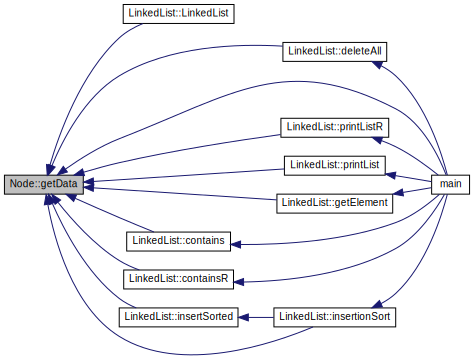
\includegraphics[width=350pt]{class_node_aca98907146d5d0687f48bf8be9df9b7d_icgraph}
\end{center}
\end{figure}
\mbox{\Hypertarget{class_node_ae36639ff267d63e058ce309fde5a9913}\label{class_node_ae36639ff267d63e058ce309fde5a9913}} 
\index{Node@{Node}!get\+Next@{get\+Next}}
\index{get\+Next@{get\+Next}!Node@{Node}}
\subsubsection{\texorpdfstring{get\+Next()}{getNext()}}
{\footnotesize\ttfamily \hyperlink{class_node}{Node} $\ast$ Node\+::get\+Next (\begin{DoxyParamCaption}{ }\end{DoxyParamCaption})}

Here is the caller graph for this function\+:
\nopagebreak
\begin{figure}[H]
\begin{center}
\leavevmode
\includegraphics[width=350pt]{class_node_ae36639ff267d63e058ce309fde5a9913_icgraph}
\end{center}
\end{figure}
\mbox{\Hypertarget{class_node_a0a2c821ab31b604e4fdd7cf39be5cc68}\label{class_node_a0a2c821ab31b604e4fdd7cf39be5cc68}} 
\index{Node@{Node}!set\+Data@{set\+Data}}
\index{set\+Data@{set\+Data}!Node@{Node}}
\subsubsection{\texorpdfstring{set\+Data()}{setData()}}
{\footnotesize\ttfamily void Node\+::set\+Data (\begin{DoxyParamCaption}\item[{int}]{data }\end{DoxyParamCaption})}

\mbox{\Hypertarget{class_node_a89b12aca90acdf6a8a547cbdab9b80a5}\label{class_node_a89b12aca90acdf6a8a547cbdab9b80a5}} 
\index{Node@{Node}!set\+Next@{set\+Next}}
\index{set\+Next@{set\+Next}!Node@{Node}}
\subsubsection{\texorpdfstring{set\+Next()}{setNext()}}
{\footnotesize\ttfamily void Node\+::set\+Next (\begin{DoxyParamCaption}\item[{\hyperlink{class_node}{Node} $\ast$}]{next }\end{DoxyParamCaption})}

Here is the caller graph for this function\+:
\nopagebreak
\begin{figure}[H]
\begin{center}
\leavevmode
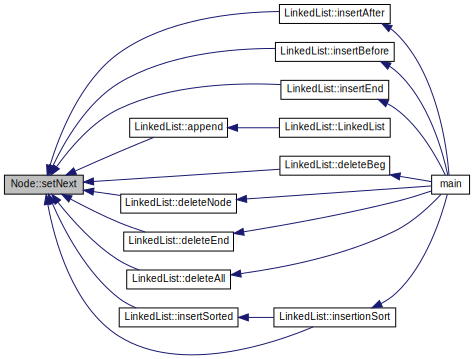
\includegraphics[width=350pt]{class_node_a89b12aca90acdf6a8a547cbdab9b80a5_icgraph}
\end{center}
\end{figure}


The documentation for this class was generated from the following files\+:\begin{DoxyCompactItemize}
\item 
D\+:/\+Git/\+Data\+Structures/\+Linked\+List/\hyperlink{_node_8hpp}{Node.\+hpp}\item 
D\+:/\+Git/\+Data\+Structures/\+Linked\+List/\hyperlink{_node_8cpp}{Node.\+cpp}\end{DoxyCompactItemize}

\chapter{File Documentation}
\hypertarget{_list_8cpp}{}\section{D\+:/\+Git/\+Data\+Structures/\+Linked\+List/\+List.cpp File Reference}
\label{_list_8cpp}\index{D\+:/\+Git/\+Data\+Structures/\+Linked\+List/\+List.\+cpp@{D\+:/\+Git/\+Data\+Structures/\+Linked\+List/\+List.\+cpp}}
{\ttfamily \#include \char`\"{}List.\+hpp\char`\"{}}\newline
Include dependency graph for List.\+cpp\+:
% FIG 0

\hypertarget{_list_8hpp}{}\section{D\+:/\+Git/\+Data\+Structures/\+Linked\+List/\+List.hpp File Reference}
\label{_list_8hpp}\index{D\+:/\+Git/\+Data\+Structures/\+Linked\+List/\+List.\+hpp@{D\+:/\+Git/\+Data\+Structures/\+Linked\+List/\+List.\+hpp}}
{\ttfamily \#include $<$iostream$>$}\newline
{\ttfamily \#include $<$climits$>$}\newline
{\ttfamily \#include \char`\"{}Node.\+hpp\char`\"{}}\newline
Include dependency graph for List.\+hpp\+:
% FIG 0
This graph shows which files directly or indirectly include this file\+:
% FIG 1
\subsection*{Classes}
\begin{DoxyCompactItemize}
\item 
class \hyperlink{class_linked_list}{Linked\+List}
\end{DoxyCompactItemize}

\hypertarget{main_8cpp}{}\section{D\+:/\+Git/\+Data\+Structures/\+Linked\+List/main.cpp File Reference}
\label{main_8cpp}\index{D\+:/\+Git/\+Data\+Structures/\+Linked\+List/main.\+cpp@{D\+:/\+Git/\+Data\+Structures/\+Linked\+List/main.\+cpp}}
{\ttfamily \#include $<$iostream$>$}\newline
{\ttfamily \#include \char`\"{}List.\+hpp\char`\"{}}\newline
Include dependency graph for main.\+cpp\+:
% FIG 0
\subsection*{Functions}
\begin{DoxyCompactItemize}
\item 
int \hyperlink{main_8cpp_ae66f6b31b5ad750f1fe042a706a4e3d4}{main} ()
\end{DoxyCompactItemize}


\subsection{Function Documentation}
\mbox{\Hypertarget{main_8cpp_ae66f6b31b5ad750f1fe042a706a4e3d4}\label{main_8cpp_ae66f6b31b5ad750f1fe042a706a4e3d4}} 
\index{main.\+cpp@{main.\+cpp}!main@{main}}
\index{main@{main}!main.\+cpp@{main.\+cpp}}
\subsubsection{\texorpdfstring{main()}{main()}}
{\footnotesize\ttfamily int main (\begin{DoxyParamCaption}{ }\end{DoxyParamCaption})}

Here is the call graph for this function\+:
% FIG 1

\hypertarget{_node_8cpp}{}\section{D\+:/\+Git/\+Data\+Structures/\+Linked\+List/\+Node.cpp File Reference}
\label{_node_8cpp}\index{D\+:/\+Git/\+Data\+Structures/\+Linked\+List/\+Node.\+cpp@{D\+:/\+Git/\+Data\+Structures/\+Linked\+List/\+Node.\+cpp}}
{\ttfamily \#include \char`\"{}Node.\+h\char`\"{}}\newline
Include dependency graph for Node.\+cpp\+:
% FIG 0

\hypertarget{_node_8hpp}{}\section{D\+:/\+Git/\+Data\+Structures/\+Linked\+List/\+Node.hpp File Reference}
\label{_node_8hpp}\index{D\+:/\+Git/\+Data\+Structures/\+Linked\+List/\+Node.\+hpp@{D\+:/\+Git/\+Data\+Structures/\+Linked\+List/\+Node.\+hpp}}
This graph shows which files directly or indirectly include this file\+:
% FIG 0
\subsection*{Classes}
\begin{DoxyCompactItemize}
\item 
class \hyperlink{class_node}{Node}
\end{DoxyCompactItemize}

%--- End generated contents ---

% Index
\backmatter
\newpage
\phantomsection
\clearemptydoublepage
\addcontentsline{toc}{chapter}{Index}
\printindex

\end{document}
